\documentclass[11pt,a4paper]{article}

\usepackage{fullpage}
\usepackage[utf8]{inputenc}
\usepackage[russian]{babel}
\usepackage{graphicx}
\usepackage{float}
\usepackage[stable]{footmisc}
\usepackage{caption}
\usepackage{subcaption}
\usepackage{url}
\setcounter{section}{-1}

\setlength\parindent{0pt}

\title{Конспект по проектированию ПО \\ \vspace{2 mm} {\large v0.1}}
\date{}

\begin{document}
\maketitle
\tableofcontents

\section{Disclaimer}
Это конспект по курсу «Проектирование программного обеспечения», прочитанному year2011 в осеннем семестре. Автор конспекта была на всех парах, на которых был и преподаватель\footnote{Дмитрий Юрьевич Кочелаев}, кроме одной (на которой, по счастливому стечению обстоятельств, лекции не было). В этом документе местами сказано больше, чем было на лекциях (так как он является жалкой попыткой автора подготовиться к сдаче зачёта), но местами — меньше (так как эти места были относительно лирическими отступлениями на лекциях, которые в общем и в целом вписываются в тему, но в ответе на вопрос смотрятся не к месту), так что его можно считать отрефакторенным конспектом, не покрытым тестами\footnote{Если вы не поняли последние пять слов, то поймёте после прочтения шестой главы.}. Дословная точность цитат не гарантируется, но никаких распятых мальчиков тут нет.

Конспект лежит по адресу \url{https://github.com/katyatitkova/software-design-outline}.

TODO: 
\begin{itemize}
\item картинки к паттернам;
\item многослойная архитектура
\end{itemize}

\section{Порождающие паттерны\footnote{На самом деле, здесь почти всё взято из книжки}}
Книжка по паттернам — конечно же, Банда Четырёх\footnote{Ralph Johnson, John Vlissides, Richard Helm, and Erich Gamma ``Design Patterns: Elements of Reusable Object-Oriented Software''}
\subsection{Singleton}
Гарантирует, что у класса есть только один экземпляр, и предоставляет ему глобальную точку доступа.

\subsection{Pool\footnote{Как ни странно, его нет в GoF}}
Храним объекты готовыми к использованию: когда нужен, берём из пула (а не создаём), когда не нужен — возвращаем в пул (а не удаляем). Pool объектов никогда нельзя писать самому.

\subsection{Builder}
Отделяет конструирование сложного объекта от его представления: в результате одного и того же процесса конструирования могут получаться разные представления.

\subsection{Prototype}
Задаёт виды создаваемых объектов с помощью экземпляра-прототипа и создаёт новые объекты, копируя этот прототип.

Используем, когда нужно много одинаковых объектов: например, в текстовом редакторе отрендерили один раз букву и юзаем. А ещё существует извращённый прототип с наследованием.

\subsection{Factory Method}
Определяет интерфейс для создания объекта, но оставляет подклассам решение о том, какой класс инстанцировать. Позволяет делегировать инстанцирование подклассам.

\subsection{Abstract Factory}
Фабрика фабрик. Предоставляет интерфейс для создания семейств взаимосвязанных или взаимозависимых объектов, не специфицируя их конкретных классов.

%\begin{figure}[H]
%\centering
%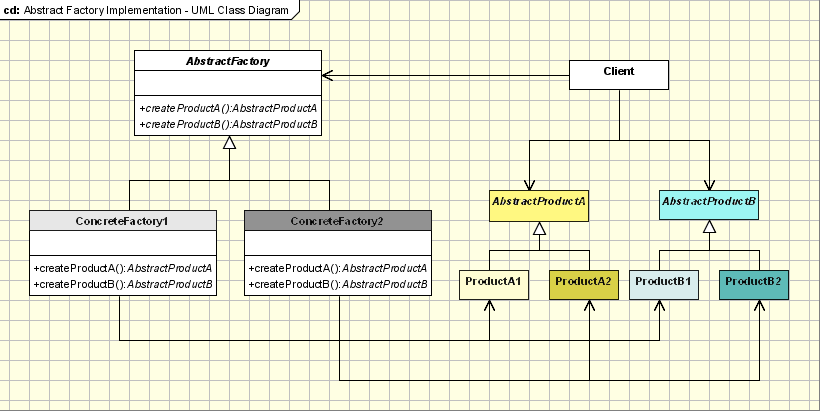
\includegraphics[width=550pt]{pics/abstract-factory-pattern.png}
%\end{figure}

\section{Структурные паттерны\footnote{И тут тоже}}
\subsection{Adapter}
Чтоб скрестить ежа с ужом: для юзания классов, не совместимых по интерфейсу.

\subsection{Bridge}
Отделяет абстракцию от её реализации так, чтобы их можно было изменять независимо.

\subsection{Composite}
Компонует объекты в древовидные структуры для представления иерархий часть-целое. Позволяет клиентам единообразно трактовать индивидуальные и составные объекты.

\subsection{Facade}
Предоставляет унифицированный интерфейс вместо набора интерфейсов подсистемы. Определяет интерфейс более высокого уровня для упрощения использования подсистемы. Если нет планов переписать, расширить, etc., то фасад не нужен.

\subsection{Decorator}
Динамически добавляет объекту новые обязанности. Является альтернативой порождению подклассов с целью расширения функциональности.

\section{Многослойная архитектура}
\begin{figure}[H]
	\centering
	\begin{minipage}{.3\textwidth}
		\centering
		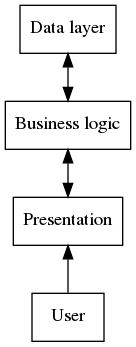
\includegraphics[width=70pt]{pics/layers.png}
		\captionof{figure}{Классика}
		\label{fig:layers}
	\end{minipage}%
	\begin{minipage}{.3\textwidth}
		\centering
		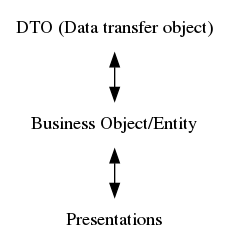
\includegraphics[width=130pt]{pics/dto.png}
		\captionof{figure}{1 layer — 1 object}
		\label{fig:dto}
	\end{minipage}
	\begin{minipage}{.35\textwidth}
		\centering
		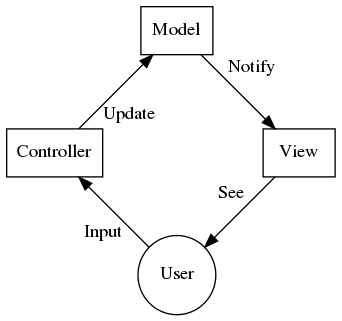
\includegraphics[width=180pt]{pics/mvc.png}
		\captionof{figure}{MVC}
		\label{fig:dto}
	\end{minipage}
\end{figure}

Казалось бы, по классической картинке всё понятно. Business logic может разрастаться вертикально.

\begin{enumerate}
\item 1 layer — 1 object

DTO — это объект, который используется для передачи данных между слоями. Сокращает количество запросов, которые обычно дороги.
\item All layers — 1 object\footnote{Кажется, никто из тех, кто ходил, не помнит, что это :( Читающий, если ты помнишь — допиши сам или расскажи Титковой!}
\end{enumerate}

Дальше было что-то про ORM.

MVC (Model-view-controller)

\section{Inversion of Control \& Dependency Injection}
Реализация принципа ``Don't call us, we'll call you''. Например, была консольная программка, которая складывала числа, которая говорила: «введите a», «введите b» (то есть программа говорила, что делать), а теперь — программка с полями для ввода и кнопкой calculate, где можно править значения в любом порядке (то есть мы управляем).

IoC нужен, чтобы:
\begin{enumerate}
\item разделить функциональность между этапами запуска и реализации;
\item разграничить: каждый модуль занимается только своей задачей, физически нельзя залезть в чужое;
\item дать модулям полагаться на контракты.
\end{enumerate}

Способы реализации:
\begin{enumerate}
\item Dependency injection — передаём dependency (сервис) dependent object'у (клиенту), то есть сервис становится частью клиента. Весело дебагать. Из интерфейса понятно, что и как у нас с клиентом.
\item Service locator — сами ищем сервис, который отвечает за нашу функциональность. Гораздо проще реализовать (в примитиве — HashMap), так как перекладывает часть логики на клиента, но значительно сложнее протестировать. В использовании зависим от интерфейса.
\end{enumerate}

Подходы к конфигурации DI:
\begin{enumerate}
\item inline (прямо в коде);
\item configs (xml, json…);
\item annotation.
\end{enumerate}

DI ещё даёт возможность использовать прокси и аспекты.

AOP (aspect-oriented programming)

Аспект — некий модуль, который реализует сквозную функциональность (функциональность, которую нельзя выделить в отдельные сущности; её реализация распределена по различным модулям программы).

Advice (совет) — дополнительная функциональность, которую хотим внести в код.

Injection point (join point) — то место, где следует применить advice.

\section{Message Queue}
Message queue — способ подружить два и более приложений. До этого были CORBA\footnote{Common Object Request Broker Architecture}, OLE\footnote{Object Linking and Embedding}, WS\footnote{Web Service(?)}.

Пример: рассылаем смс о транзакциях в банке.

\begin{figure}[H]
	\centering
	\begin{minipage}{.5\textwidth}
		\centering
		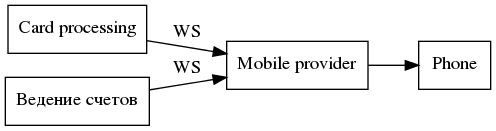
\includegraphics[width=200pt]{pics/ws.png}
		\captionof{figure}{Плохая схема}
		\label{fig:ws}
	\end{minipage}%
	\begin{minipage}{.5\textwidth}
		\centering
		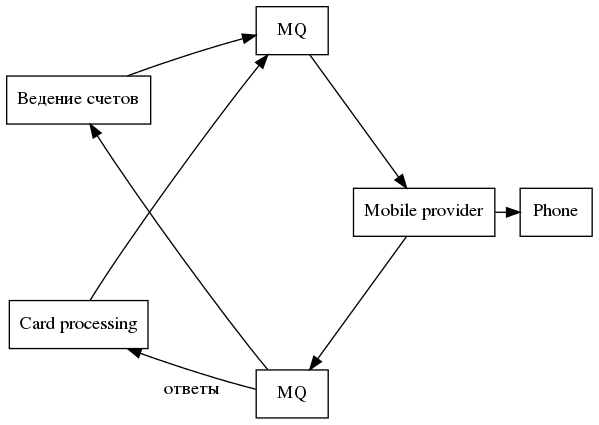
\includegraphics[width=230pt]{pics/mq.png}
		\captionof{figure}{Хорошая схема}
		\label{fig:mq}
	\end{minipage}
\end{figure}

У нас есть какая-то пропускная способность для отправки смсок. Первого числа всем начислили зарплату, пошёл поток смсок. При плохой схеме у нас висят транзакции, по которым ещё не отправились. При хорошей мы завершили транзакцию, отправив смску в очередь.

Очередь должна уметь восстанавливаться, поэтому мы делаем их три. Ответ «ок» на клиенте, когда мы положили сообщение во все очереди. Зачем три? Если одна умерла, то по тому, есть ли сосед, понимаем, мы умерли или не мы\footnote{«Кто не смотрел ``Шестое чувство'': это был спойлер»}

Гарантии доставки:
\begin{itemize}
\item at least once — доставляем минимум один раз, чтоб гарантированно получить ответ;
\item at most once — доставляем максимум один раз (выполнить операцию дважды хуже, чем не выполнить вообще).
\end{itemize}

\begin{figure}[H]
	\centering
	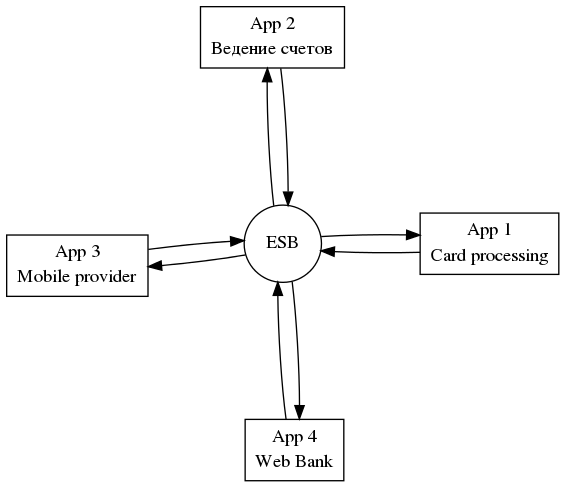
\includegraphics[width=200pt]{pics/bus.png}
	\caption{(Enterprise) Service Bus. Стрелочки чаще всего — очереди}
\end{figure}

В очередях плохо хранить большие сообщения, поэтому обычно header хранят в очереди, а binary data — в file storage.

\section{Рефакторинг}
По рефакторингу есть классическа книжка Фаулера\footnote{Martin Fowler ``Refactoring: Improving the Design of Existing Code''}. ДК говорит, что Фаулер считает, что «жить без рефакторинга так же сложно, как без Крыма». И советует для общего образования пролистать оглавление, а если есть куча свободного времени — почитать. Но от него хорошо засыпается\footnote{…и поэтому автор только пролистала. Там действительно разобраны довольно очевидные проблемы с довольно очевидными путями решения.}.

Рефакторить можно код, структуру БД, интерфейсы.

\subsection{Рефакторинг кода}
Preconditions для рефакторинга кода с точки зрения Фаулера (не ДК):
\begin{itemize}
\item добавляется новая функциональность;
\item исправление ошибок («как если криво висела картина, а мы заодно обои переклеили»);
\item изучение кода («самое страшное», «как если висит полочка, вытащили её, снова переклеили обои, пролили клей на паркет, переложили его, а попутно сломали кафель в ванной…»)
\end{itemize}

Да, «рефакторинг — как ремонт». Вообще, «первые два пункта имеют право на жизнь», а «новая функциональность без рефакторинга — как балконы в Молдавии»\footnote{Дальше был рассказ ДК о том, что в Молдавии любят достраивать балконы вперёд, причём балконы третьего этажа опираются на достроенные балконы второго и так далее.}, но «надо было переклеить одно полотнище — не надо перекладывать кафель у соседей».

Для рефакторинга нужен хороший coverage тестами, но тесты-то тоже переделаются…

Test-driven development, с точки зрения ДК, гиблый метод. «Есть тесты, и нет ничего. Обычно в этот момент сдавать надо». Раз сразу всё обложили тестами, то придумали и интерфейс, а он всё равно десять раз перепишется, пока будем писать код.

Кстати, выкинуть старое, написать новое — не рефакторинг.

Если у нас coverage тестами $95\%$, то можно не рефакторить функцию на 15 экранов. А развернуть цикл иногда ок: например, если это цикл до $4$, занимающийся получением byte'ов из int'а, так понятнее будет.

Советы ДК по поводу рефакторинга кода:
\begin{itemize}
\item не рефакторить просто так;
\item рефакторить, только если обложили всё тестами;
\item сразу писать так, чтобы не рефакторить;
\item полезный рефакторинг — в процессе написания.
\end{itemize}

\subsection{Рефакторинг БД}
Рефакторинг БД и интерфейсов — занятие мрачное и неблагодарное. Принципиальное отличие рефакторинга БД от рефакторинга кода — нет тестов для структуры БД, у всех всё может работать, но неправильно. Добавить новую колонку не страшно, обычно не ломает старое, а вот расширение поля — ой.

Советы от ДК:
\begin{itemize}
\item пытаться писать тесты на БД;
\item спроектировать сразу хорошо.
\end{itemize}

\subsection{Рефакторинг интерфейсов}
После рефакторинга интерфейса все пользователи нашей библиотеки нас люто ненавидят. Правильно делать так: 

\begin{enumerate}
\item выкатываем новый API в sandbox (в котором работают оба, можно их посравнивать между собой);
\item в продакшне работают оба API (причём хорошо сделать такой ключ, что все, кто получил его после выхода нового, не могут использовать старый);
\item можно убить старый (отвалятся примерно $15\%$ приложений, использующих его, из них $50\%$ ничего не заметят, $15\%$ напишут гневное письмо, но ничего не сделают, остальные как-то приспособятся).
\end{enumerate}

А за рефакторинг как самоцель надо бить.

\end{document}